\documentclass[paper=letter, fontsize=11pt]{scrartcl} 
\usepackage{graphicx}
\usepackage{verbatim}
\usepackage{pictex}  
\usepackage{multimedia}
\usepackage{listings}
\usepackage{xcolor,colortbl}
\usepackage[utf8]{inputenc}		%para identificar acentos(encoding)
\usepackage{url}
\usepackage[spanish]{babel} % language/hyphenation
\usepackage{amsmath,amsfonts,amsthm} % Math packages
\usepackage{amsbsy}
\usepackage{amssymb}
\usepackage{fancyvrb}
\usepackage{sectsty} % Allows customizing section commands
\allsectionsfont{\centering \normalfont\scshape} % Make all sections centered, the default font and small caps
\usepackage{float}%para fijar las figuras y tablas
\usepackage{placeins}%fija espacios
\usepackage{fancyhdr} % Custom headers and footers
\pagestyle{fancyplain} % Makes all pages in the document conform to the custom headers and footers
\fancyhead{} % No page header - if you want one, create it in the same way as the footers below
\fancyfoot[L]{} % Empty left footer
\fancyfoot[C]{} % Empty center footer
\fancyfoot[R]{\thepage} % Page numbering for right footer
\renewcommand{\headrulewidth}{0pt} % Remove header underlines
\renewcommand{\footrulewidth}{0pt} % Remove footer underlines
\setlength{\headheight}{13.6pt} % Customize the height of the header

\numberwithin{equation}{section} % Number equations within sections (i.e. 1.1, 1.2, 2.1, 2.2 instead of 1, 2, 3, 4)
\numberwithin{figure}{section} % Number figures within sections (i.e. 1.1, 1.2, 2.1, 2.2 instead of 1, 2, 3, 4)
\numberwithin{table}{section} % Number tables within sections (i.e. 1.1, 1.2, 2.1, 2.2 instead of 1, 2, 3, 4)

\setlength\parindent{0pt} % Removes all indentation from paragraphs - comment this line for an assignment with lots of text

\newcommand{\horrule}[1]{\rule{\linewidth}{#1}} % Create horizontal rule command with 1 argument of height

\title{	
\normalfont \normalsize 
\textsc{Centro de Investigaci\'on en Matem\'aticas (CIMAT). Unidad Monterrey} 
\\ [25pt] 
\horrule{0.5pt} \\[0.4cm] % Thin top horizontal rule
\huge Ciencia de datos (Tarea 4) \\ 
\horrule{2pt} \\[0.5cm] % Thick bottom horizontal rule
}

\author{José Antonio Garcia Ramirez} % Your name

\date{\normalsize\today} % Today's date or a custom date

\begin{document}
\lstdefinestyle{customc}{
  belowcaptionskip=1\baselineskip,
  basicstyle=\footnotesize, 
  frame=lrtb,
  breaklines=true,
  %frame=L,
  %xleftmargin=\parindent,
  language=C,
  showstringspaces=false,
  basicstyle=\footnotesize\ttfamily,
  keywordstyle=\bfseries\color{green!40!black},
  commentstyle=\itshape\color{red!40!black},
  identifierstyle=\color{blue},
  stringstyle=\color{purple},
}

\lstset{breakatwhitespace=true,
  basicstyle=\footnotesize, 
  commentstyle=\color{green},
  keywordstyle=\color{blue},
  stringstyle=\color{purple},
  language=C++,
  columns=fullflexible,
  keepspaces=true,
  breaklines=true,
  tabsize=3, 
  showstringspaces=false,
  extendedchars=true}

\lstset{ %
  language=R,    
  basicstyle=\footnotesize, 
  numbers=left,             
  numberstyle=\tiny\color{gray}, 
  stepnumber=1,              
  numbersep=5pt,             
  backgroundcolor=\color{white},
  showspaces=false,             
  showstringspaces=false,       
  showtabs=false,               
  frame=single,                 
  rulecolor=\color{black},      
  tabsize=2,                  
  captionpos=b,               
  breaklines=true,            
  breakatwhitespace=false,    
  title=\lstname,             
  keywordstyle=\color{blue},  
  commentstyle=\color{dkgreen},
  stringstyle=\color{mauve},   
  morekeywords={\%*\%,...}         
} 


\maketitle % Print the title

\section{Ejercicio 1}

\textit{Aunque hay varias extensiones de AdaBoost al caso multiclase, una de las más usadas es la llamada SAMME (Stagewise Additive Modeling using a Multi-class Exponential loss
function), ya que está basada en la caracterización estadística de Friedman et al. Implementa esta versión de AdaBoost y verifica su desempeño en un conjunto de datos con más de dos categorias.\\}

El código de la implementación del algoritmo adaboost para el caso multicase se anexa en el archivo ‘ejercicio1.R’, la implementación sigue fielmente el algoritmo 2 SAMME del mencionado paper. \\

A Diferencia del paper, donde se menciona que los clasificadores débiles de Adaboost fueran árboles que tuviesen el mismo número de nodos terminales, a pesar de que mencionan que este parámetro se determinó por validación cruzada, en nuestros resultados se reportan los parámetros de máxima profundidad de los árboles y el número mínimo de elementos en cada rama.\\

Primero consideramos el conjunto de datos simulados que los autores del paper nombran como ‘Waveform’, originados como se menciona en el paper partiendo de combinaciones lineales  de muestras uniformes con otras variables triangulares y a las que se les agrega ruido blanco. En la figura 1.1 podemos ver la disminución del error conforme el número de árboles se incrementa. Para este escenario se buscó afinar tanto el parámetro \textit{maxdepth} y \textit{minisplit} sin embargo sólo reportamos los mejores desempeños en el conjunto de prueba, por ejemplo con los parámetros de $maxdepth=20, minisplit=3$ y con 600 clasificadores débiles se obtuvó un $32.1\%$ de error en el conjunto de prueba.    \\

\begin{figure}[H]
  \begin{center}
    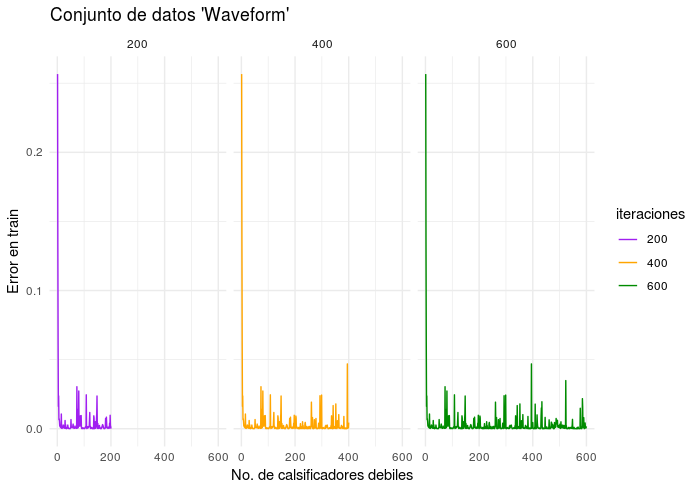
\includegraphics[width=12cm]{error_waveform_train.png}
    \caption{Error en el conjunto de prueba ‘Waveform’ conforme se utilizan más clasificadores débiles. Los parámetros fueron $maxdetp=12, minsplit = 10$ y el número de clasificadores débiles, 200 (izquierda), 400 (centro) y 600 (derecha).   }
    \label{figura1_1}
  \end{center}
\end{figure}
\FloatBarrier

Posteriormente utilizamos el conjunto de que los autores del paper usaron y que consideraron como el más desafiante, ‘Vowels’ disponible en el sitio web de UCI: Center for machine learning and intelligent systems.
Características importantes de los conjuntos de datos se presentan en el cuadro 1.1. y el desempeño de nuestra implementación vs la citada en el paper en el cuadro 1.2\footnote{Ellos reportan el error medio con su desviación en nuestro caso solo reportamos el error de una ejecución aleatoria pero con semilla fija.}.\\

En la figura 1.2 podemos ver la disminución del error conforme el número de árboles se incrementa para el algoritmo sobre el conjunto de datos ‘Vowels’. Para este escenario se buscó afinar tanto el parámetro \textit{maxdepth} y \textit{minisplit} sin embargo sólo reportamos los mejores desempeños en el conjunto de prueba, por ejemplo con los parámetros de $maxdepth=10, minisplit=10$ y con 600 clasificadores débiles se obtuvó un $44.8\%$ de error en el conjunto de prueba.    \\
En este caso el conjunto de entrenamiento y el conjunto de prueba están definidos por una variable del conjunto de datos.
\begin{figure}[H]
  \begin{center}
    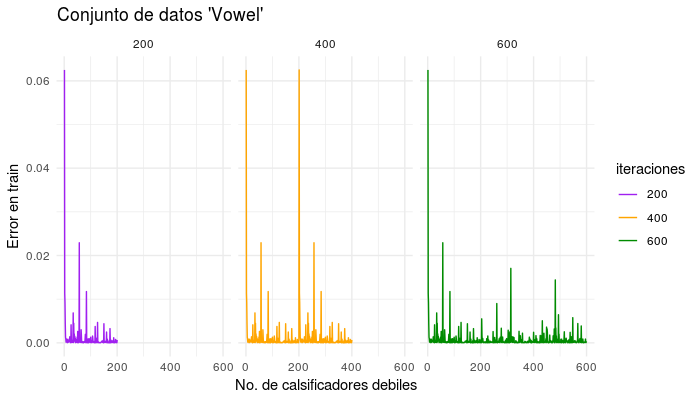
\includegraphics[width=12cm]{vowel_error_train.png}
    \caption{Error en el conjunto de prueba ‘Vowel’ conforme se utilizan más clasificadores débiles. Los parámetros fueron $maxdetp=12, minsplit = 10$. 
Los colores corresponden con los mismos de la figura 1.1 }
    \label{figura1_2}
  \end{center}
\end{figure}
\FloatBarrier

\begin{minipage}{\linewidth}
\centering
\begin{tabular}{l|c|c|c|c}\hline
Conjunto de datos  & \# obs. de entrenamiento & \# obs. de prueba  & Variables & Clases \\ \hline
Waveform & 300 & 4998 & 1 & 3 \\
Vowel & 528 & 462 & 10 & 11\\ \hline
\end {tabular}
\captionof{table}{Características de los conjuntos de datos sobre los que se probó la implementación de Adaboost multiclase. }
\label{descripcion} 
\end{minipage}


\begin{minipage}{\linewidth}
\centering
\begin{tabular}{l|ccc}\hline
 & \# iteraciones & (error en  & prueba)  \\ \hline
Método  & 200 & 400 & 600\\ \hline
\textbf{Waveform} & & & \\
Adaboost propio & 65.5& 65.5 & 65.5\\
SAMME\footnote{Valores reportados en el paper} & 16.5 & 16.4& 16.3\\ \hline
\textbf{Vowel} & & & \\
Adaboost propio & 43.2 & 44.5 & 42.8 \\
SAMME& 43.9 & 43.3& 43.3\\ \hline
\end {tabular}
\captionof{table}{Desempeño de nuestra implementación contra la reportada en el paper en los conjuntos de datos que consideramos. Para el conjunto ‘Wameform’ los parámetros fueron $maxhdeth=12,minsplit = 3$, para el ‘Vowels’ fueron $maxhdeth=12,minsplit = 10$. }
\label{resultados} 
\end{minipage}
\FloatBarrier 
\[\]
\textit{Incluye una breve descripción del método basandote en el artículo: Zhu J, Zou H, Rosset S, and Hastie T (2009). Multi-Class AdaBoost. Statistics and Its Interface,2, 349360. Puedes
usar también los datos que ahí se muestran para reproducir los resultados.}\\

De manera análoga a como lo vimos en clase e inclusive podríamos decir pretenciosamente que la extensión de Adaboost al caso multiclase es natural. Si bien se parte como en la mayoría de métodos de clasificación definiendo una función de pérdida $L(y,f) = exp^{(-\frac{1}{K} (y_1 + … +y_kf_f)}$  donde las $y_i$ son las etiquetas de nuestro conjunto de entrenamiento y buscando minimizar el costo. El detalle, al igual que en el caso de dos clases, recae en que esta minimización es en el espacio de funciones\footnote{Pues estamos buscando una función $f$ que minimice el costo}. Con un curioso encoding que consiste en hacer vectores de dimensión $k$ para cada etiqueta, se realiza la búsqueda de la función $f$ (al igual que en muchos métodos de optimización obteniendo el gradiente y siguiéndolo en su dirección negativa) sin embargo lo delicado recae en asumir que la función $f$ cumple una recurrencia o bien que de manera iterativa podremos construirla de la forma $f (x) = \sum_{i=1}^n \beta^{(m) }g^{(m)}(x)$, donde es importante notar que las funciones $g(x)^{(m)}$ son una base del subespacio en donde se está buscando la solución. Como nota importante estas funciones $g^{(m)}$ deben de ser linealmente independientes y lo curioso de esta formulación y derivación es que me parece que conlleva a aceptar el axioma de elección (para poder tener el resultado de que cualquier espacio vectorial posee una base, inclusive los de dimensión infinita) \footnote{Sin embargo no he encontrada ningún detalle en el paper que toque el tema}. Estas funciones $g(x) ^{(m)}$ a su vez construyen iterativamente a la función $f$, pues se cumple que $f^{(m)}(x) =f^{(m-1)}(x)+\beta^{(m)}g^{(m)}(x)$ y las funciones  $g(x)^{(m)}$ se corresponden con nuestros clasificadores débiles. \\

Hasta aquí la diferencia con el caso biclase es ‘mínima’ pues solo se cambio la función de costo y se actualizaron los cálculos que involucra actualizar los tamaños de paso en el descenso del gradiente. Lo que es importante es que en la sección del paper 2.2 \textit{The multi-class exponential loss} se prueba que al encontrar la función $f$, de la que hemos estado hablando, coincide con la regla de clasificación de Bayes ,es decir que esta función y la función de pérdida exponencial (con ese ligero término de diferencia $log(k-1)$) le otorgan al método la característica de ser Fisher consistente en la versión multiclase, no solo con la función logit sino la exponencial y la $L_2$.\\
Como conclusión de este ejercicio hacemos notar que tuvimos que incrementar el nivel de profundidad de los clasificadores débiles para competir con los resultados del paper. Puede que esto haga que ya no sean clasificados como débiles pero fue necesario en principio para garantizar que la probabilidad de asignar correctamente fuese mayor a $1/k$ 


\section{Ejercicio 2}
\textit{
Usando los datos de los dígitos escritos a mano y  digitalizados, complementa el ejercicio que hiciste en la tarea 1 aplicando métodos de clasificación basados en}
\begin{itemize}
\item LDA
\item QDA
\item Redes neuronales
\item Máquinas de Soporte Vectorial
\item Arboles de clasificación
\item AdaBoost
\end{itemize}
\textit{Utiliza K-Fold CV como criterio para elegir el mejor modelo, así como para compararlos. ¿Qué método elegirías?}\\

Considerando el conjunto de datos de entrenamiento y de prueba como una sola muestra implementé el método de k-Fold, con $k=10$, el método que consiste primero en crear 10 particiones iniciales entrenar con las 9 últimas y validar con la primera posteriormente entrenar con la primera y las ocho últimas y validar con la segunda etc, para entrenar y validar los errores de los métodos (incluyendo los casos en donde realicé afinamiento de los parámetros). Posteriormente considere el promedio de las precisiones en los conjuntos de entrenamiento  y prueba y es lo que reportó en la gráfica 2.1.\\

En todos los métodos considere las implementaciones de diversos paquetes de R excepto para la regresión multilineal sobre PCA (con matriz de varianzas), en este caso en la tarea 1 mostré que con 50 componentes el error de entrenamiento y de prueba no se reducía considerablemente al agregar otros pares de componentes.\\

Para los demas metodos de LDA y QDA no se requiere afinar ningun parámetro, sin embargo el QDA lo realice con los datos de PCA que genere en el ejercicio 4 de la tarea 1 esto debido a cuestiones numéricas ya que este método tiene detalles cuando hay colinealidad en los datos.\\ Para la red neuronal considere una red con una capa oculta con tres nodos lo que da aproximadamente $257 \times 3 $ aristas, esto por temas de interpretabilidad. Para las SVMs realice una búsqueda sobre un grid formado por 15 puntos igualmente espaciados en el rango $[0.1, 20]$ (las gráficas sobre la afinación de los parámetros para SVM, árboles y adaboost las incluyo en el segundo tab de la aplicación Shiny que anexo en la subcarpeta ‘Appactualizada’ de la carpeta  ‘Ejercicio2’ donde además incluyo el código correspondiente a este análisis llamado ‘ejercicio2.R’) para SVM el mejor parámetro $C$ de penalización que encontré fue de $0.1$. Para el caso del árbol realice una búsqueda sobre los pares $(maxdepth,minsplit)$ en el grid formado $\{1,2,3,...,15\} \times \{5,10,15,20\}$ el conjunto de parámetros con mejor desempeño después de k-Fold fueron $(15,20 )$. Finalmente para el adaboost realice una búsqueda de las tripletas $(minsplit, maxdepth, no.iteraciones)$ en el grid formado por  $(  5,7,9,11,...,19) \times (5,10,15) \times ( 50,100,500)$ en este caso el punto en el espacio de hiperparametros de mejor desempeño fue $(9,10,50)$.\\
Como podemos apreciar en la figura 2.1, la red neuronal tiene mayor varianza en su precisión usando k-fold, al igual que adaboost en donde en la mayoría de las particiones el ajuste fue malo, esto contrasta con la teoría de adaboost\footnote{se puede deber a una mala implementación o a que en el grib sobre el que se buscaron los mejores parámetros no considero un número suficientemente grande de iteraciones}.\\
Todos los clasificadores tienen aproximadamente el mismo error en ambos conjuntos. Se destaca la superioridad de la implementación de QDA que realizamos la cual utiliza las primeras 50 componentes principales, si bien computacionalmente esto es menos costoso que el problema de optimización de SVM, \textbf{prefiero el clasificador SVM} ya que muestra menor varianza en los casos prueba y aunque su complejidad en tiempo es mayor a la del QDA aquí implementado en nuestros experimentos es mucho más rápido que Adaboost y requiere de menos parámetros que afinar.
Como ya lo mencione he actualizado mi app, la cual anexo en la subcarpeta ‘AppActualizada’ de la tarjeta ‘ejercicio2’ donde también incluyó visualizaciones sobre el afinamiento de parámetros para Adaboost, SVM y los modelos de árboles. La aplicación utiliza los ya definidos modelos para entrenar.\\



\textit{Especifica los parámetros que usaste en cada método de clasificación. Incluye gréficos informativos sobre el desempeño de cada método. Actualiza tu aplicación interactiva, si es que la implementaste en la primera tarea.}

\begin{figure}[H]
  \begin{center}
    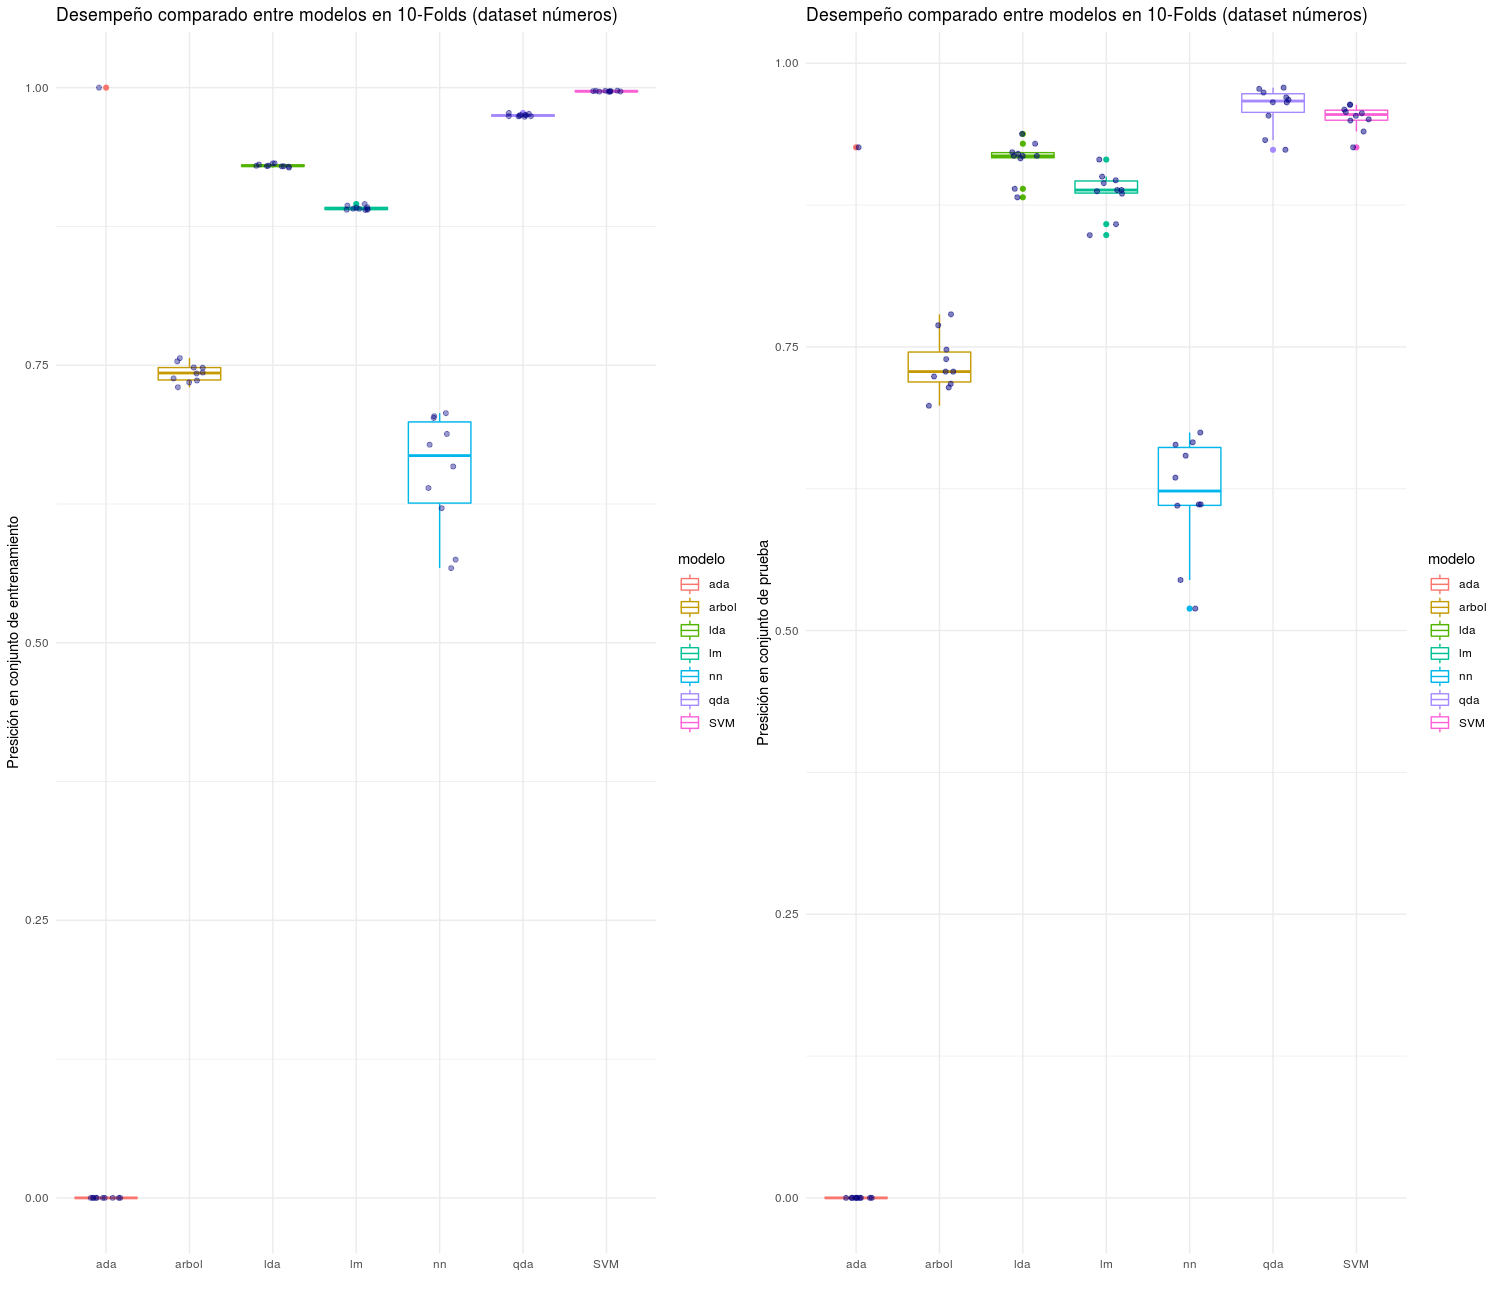
\includegraphics[scale =.35]{comparacionmodelos.png}
    \caption{Error en los conjunto de dígitos  de prueba y entrenamiento usando validación 10-Fold usando diferentes clasificadores. Los puntos representan cada una de las 10 ejecuciones de k-fold }
    \label{figura1_2}
  \end{center}
\end{figure}
\FloatBarrier

\section{Ejercicio 3}
\textit{Repite el ejercicio 2 para los datos de frutas que usaste en la tarea 2. Utiliza la representación en el espacio HSV con la mediana y los cuartiles centrales.} \\

Tal cual como lo pide el ejercicio rehice el ejercicio 2. Lo que me llevó de nuevo a escoger un número correcto de componentes para el primer método, y si mejora su desempeño para usarlo con QDA.  En la gráfica 3.1 se muestra que esta elección no era tan difícil como en el caso anterior, pues la dimensión con la que estamos tratando es mucho menor, consideré que con dos componentes basta para trabajar pues es uno de los curiosos casos en que un número pequeño de componentes el error de entrenamiento y de prueba se interceptan.
\begin{figure}[H]
  \begin{center}
    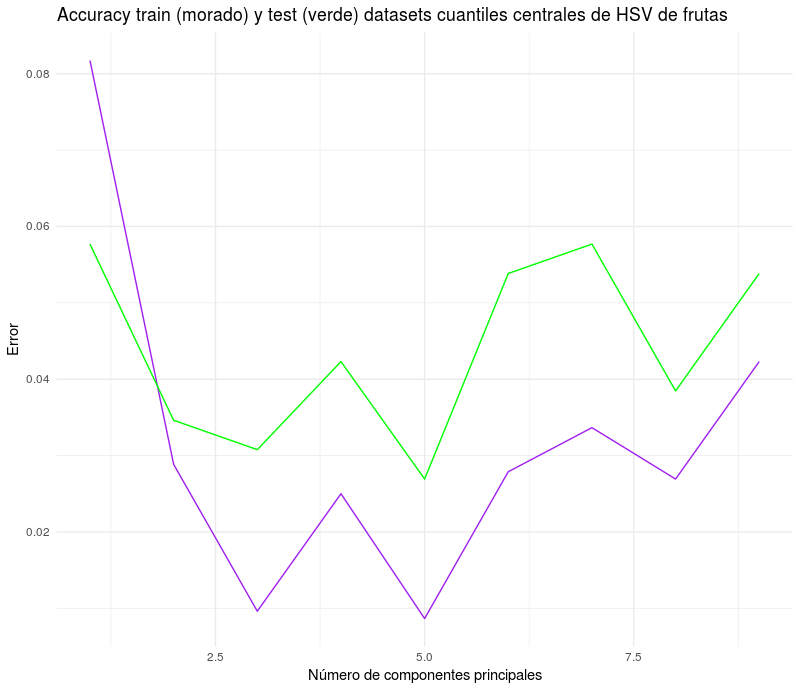
\includegraphics[scale =.40]{errores_para_nueva_p.png}
    \caption{Error contra el número de componentes usadas en el conjunto de cuartiles centrales de las imágenes de frutas. }
    \label{figura1_2}
  \end{center}
\end{figure}
\FloatBarrier
Al igual que en el ejercicio utilice QDA sobre los datos de las dos primeras componentes. Para la red neuronal de una capa oculta utilize 30 nodos, esto en vista de que la implementación lo puede trabajar (y esperando ver un sobre ajuste) para los modelos de SVM, los árboles y adaboost realice una búsqueda en grids. 

Con la misma notación para el conjunto de vectores el grid en el que busque para SVM consistió en $\{0.1, 10.1, 20.1, ...,190.1\}$ donde el mejor punto fue $C=190.1$, sin embargo en buscar numero mayores para $C$ el desempeño no mejoró. con lo que entrene el algoritmo.\\

Para el caso de los árboles estos fueron sumamente dificiles de ajustar, se consideraron varios grid, el grid menos vergonzoso consistio en $\{1,10,30\}\times\{1,2,...,10\}$ donde en todos los puntos del grid se logro un error de entrenamiento de menos de 0.5 y 0 en el conjunto de prueba . Y finalmente para Adaboost el entrenamiento fue sencillo, frente a los árboles, el grid de búsqueda se $\{5,7,9,..., 19\}\times \{5,10,15\} \times \{50,100,500\}$. Hubo varios puntos del grid con desempeño casi identico nosotros usaremos como referente el punto $(5,5,500)$ para las ejecuciones.
De la imagen 3.2, podemos ver que la red neuronal tiene un sobre ajuste pues sus errores en el conjunto de entrenamiento son muy bajos, pues su precisión es alta, sin embargo para el conjunto test presenta gran varianza y en promedio una precisión menor a nuestro favorito SVM y a los árboles. Es de destacarse que aunque los árboles son conceptualmente sencillos en la práctica ajustar sus parámetros me fue difícil. Nuevamente doy mi voto de mejor desempeño en este conjunto de datos de baja dimensión a SVM, e inclusive en el punto anterior con una dimensión de 256 aprox. se desempeñó bien en parte debido a los tamaños de prueba. Así que con el modelo entrenado de SVM con los parámetros encontrados procederá a evaluar las imagenes que saque las cuales se encuentran en la subcarpeta  ‘frutas propias’ de la carpeta ‘ejercicio 3’. Sin embargo dada la baja calidad de segmentación que logre y las diferencias de luz no espero mejores resultados. 


\begin{figure}[H]
  \begin{center}
    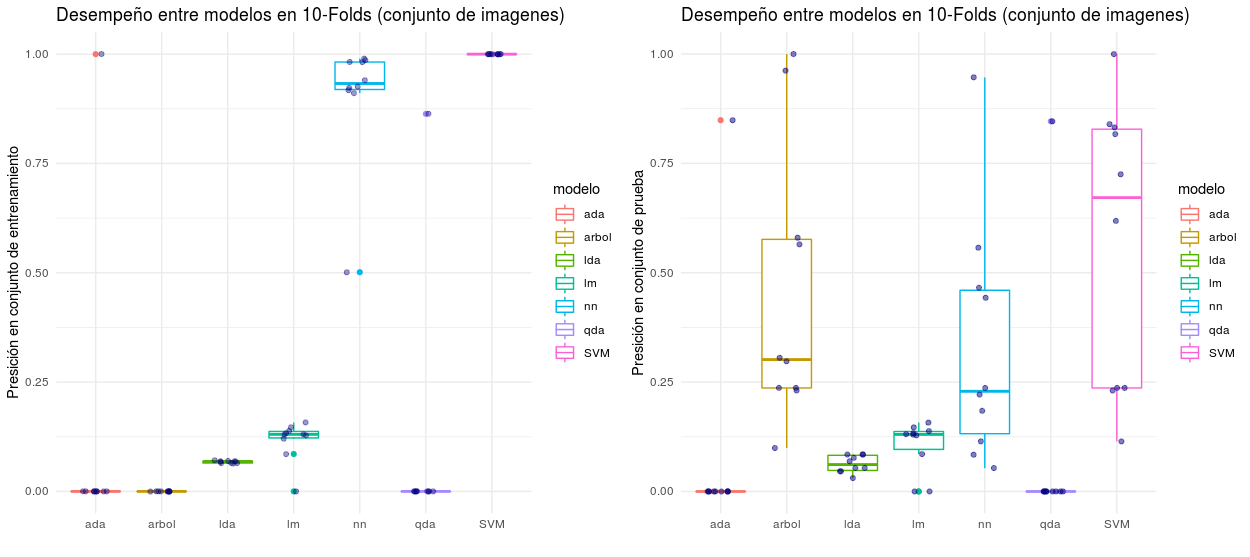
\includegraphics[scale =.5]{imagenesmodelos.png}
    \caption{Error en los conjunto de imagenes de frutas de prueba y entrenamiento usando validación 10-Fold con diferentes clasificadores. Los puntos representan cada una de las 10 ejecuciones de k-fold.}
    \label{figura3_2}
  \end{center}
\end{figure}


\textit{ Puntos extra: verifica el desempeño en del clasificador que elegiste en ejemplos 'reales'. Toma algunas fotos de frutas y realiza un preprocesamiento básico para clasificarlas. Puedes
usar el código en C (cortesía de Karen) para quitar el fondo de tu foto. Leé las instrucciones que vienen documentadas.\\
¿Cómo funciona tu clasificador? ¿Qué tan sensible es a las condiciones de la imagen (tamaño, rotación, etc.)?}\\\\
Para los puntos extras después de determinar qué modelo era mejor, generé mis propias imágenes. Fui al supermercado\footnote{Supermercado la Roma y agradezco al gerente Vicente Fernandez por permitirme sacar las fotos} fotografie frutas y las segmente. En principio no decidí invertir tiempo para usar opencv C en mi equipo, pues en python (desde Anaconda se instala fácilmente)\footnote{Y tuve problemas para instalarlo en mi equipo} por lo que intente aplicar el algoritmo de $Normalized Cut$ para segmentar\footnote{Con el cual ya he trabajado \url{https://www.overleaf.com/read/pnqsbjrmyhvk}}, en vista de que eran imágenes pequeñas, lo cual tampoco resultó. Finalmente en el código ‘mini\_cut\_float.R’ en la carpeta ‘ejercicio3’ se encuentra la manera en que segmenté las imágenes, la idea se basa en aprovechar el fondo blanco con el que saque las fotos y establecer un umbral basado en la media y la varianza de la imagen en escala de grises, en la misma carpeta se encuentran las imágenes, los recortes y las segmentaciones. El recorte de las imágenes originales lo realice a mano con el softeare Fiji \url{https://fiji.sc/}.\\

Las imágenes fueron tomadas con un dispositivo móvil de gama media. algunas imagenes se sacaron con flash y otras sin él (para variar las intensidades de luz) y las frutas se rotaron para tener varios ángulos de ellas.  Las imágenes corresponden a 4 fotos de una especie parecida a la etiquetada como ''Apple\_Breabur'', 6 a un fruto parecido al etiqueta como ''Apple\_Granny'', una de un aguacate, 3 de plátanos (que originalmente no están en la muestra de entrenamiento y esperamos ver cómo se clasifican según el modelo que entrenamos en la sección anterior SVM con el parámetro afinado), 3 cerezas bastante maduras, dos kiwis y 5 naranjas. Las imagenes se muestran en la figura 3.3.\\


\begin{figure}[H]
  \begin{center}
    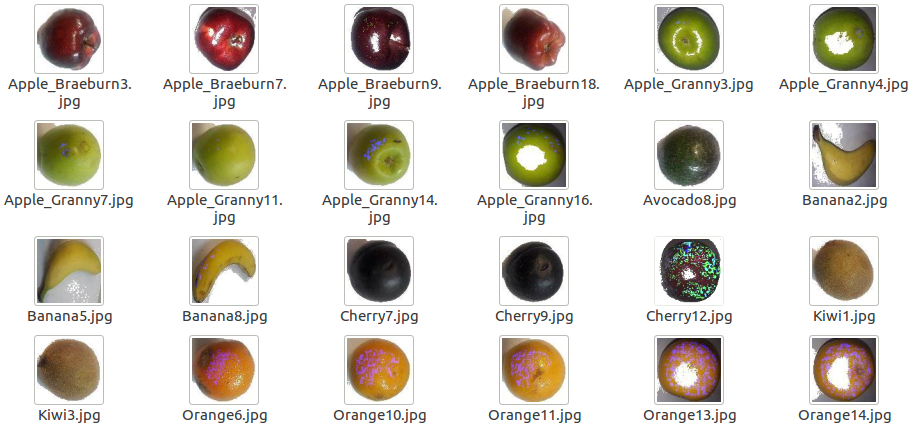
\includegraphics[scale =.5]{nuevamuestra.png}
    \caption{Imagenes de frutas segmentadas que se clasificaron con el modelo SVM elegido en la sección anterior. Notese el nombre de las imagenes que corresponde con el del cuadro 3.1}
    \label{figura3_3}
  \end{center}
\end{figure}

Los resultados, pese a todos los factores (condiciones no controladas, iluminación y modesta segmentación) no son tan desalentadores y se muestran en el cuadro 3.1

\begin{minipage}{\linewidth}
\centering
\begin{tabular}{l|c|r}\hline
   Nombre de la imagen & clasificación de SVM & Coinciden\\ \hline
   Apple\_Braeburn18.jpg &      Strawberry&  $\times$\\
   Apple\_Braeburn3.jpg  &        Avocado& $\times$ \\
   Apple\_Braeburn7.jpg   &   Huckleberry& $\times$ \\ 
   Apple\_Braeburn9.jpg &     Huckleberry& $\times$\\
    Apple\_Granny11.jpg & AppleGrannySmith& $\checkmark$\\
    Apple\_Granny14.jpg & AppleGrannySmith& $\checkmark$\\
    Apple\_Granny16.jpg & AppleGrannySmith& $\checkmark$\\
     Apple\_Granny3.jpg & AppleGrannySmith& $\checkmark$\\
     Apple\_Granny4.jpg & AppleGrannySmith& $\checkmark$\\
    Apple\_Granny7.jpg  & AppleGrannySmith& $\checkmark$\\
         Avocado8.jpg  &        Avocado& $\checkmark$\\
          Banana2.jpg  &        Avocado& $\times$\\
          Banana5.jpg  & AppleGrannySmith& $\times$\\
          Banana8.jpg  &     Strawberry& $\times$\\
         Cherry12.jpg  &        Avocado& $\times$\\
          Cherry7.jpg  &        Avocado& $\times$\\
          Cherry9.jpg  &        Avocado& $\times$\\
            Kiwi1.jpg  &           Kiwi& $\checkmark$ \\
           Kiwi3.jpg   &          Kiwi& $\checkmark$\\
         Orange10.jpg  &          Peach& $\times$\\
         Orange11.jpg  &          Peach& $\times$\\
         Orange13.jpg & AppleGrannySmith& $\times$\\
         Orange14.jpg & AppleGrannySmith& $\times$\\
          Orange6.jpg  &          Peach & $\times$\\
\end {tabular}
\captionof{table}{Clasificación efectuada por el modelo entrenado SVM sobre el conjunto de frutas de la figura 3.3.}
\label{resultados3} 
\end{minipage}
\FloatBarrier 


Como afinamos el parámetro de SVM a la par que realizamos la validación cruzada consideramos prudente tomar este modelo con $C=190.1$ y utilizar toda el conjunto de datos que se nos otorgó como conjunto de entrenamiento y como conjunto de prueba nuestras fotos. Si bien logramos una clasificación de 37.5\% con el modelo de SVM , no podemos pasar por alto algunas consideraciones como que las imágenes de manzanas verde y aguacates son fáciles de reconocer junto con los kiwis, que las cerezas son fácilmente confundibles con aguacates y que lo plátanos si se asignan aleatoriamente. Pero aun un 37\% es mejor que el 7\% que equivale a lanzar un boleto o tomar una decisión sin información ninguna.

Si bien las condiciones de luz afectan enormemente en el caso de SVM pues al trabajar en RGB habría más vectores soportes, considerando la norma euclidiana, en las que yo realice procure mantener condiciones controladas.\\
La clasificación no se ve alterada por rotaciones, pues estamos considerando los cuartiles centrales para clasificar. \\

Finalmente como recomendación para mejorar el clasificador usaría técnicas de aumentación de datos, en vista que de inicio para segmentar con NormalizedCut (el cual tiene un enfoque global) fracasó miserablemente, para captar características locales de los puntos ya que en el caso de las frutas y otros objetos deben de tener características bien determinadas, invariantes a escalas y rotaciones , como los puntos SIFT que considero que harían más sencilla la discriminación de frutas, más no la detección de maduración.\\

\section{Ejercicio 4}

\textit{Considera los datos contenidos en \textbf{img\_expression.zip}, que corresponden a fotos (256$\times$256 pixeles) de mujeres japonesas con diferentes tipos de expresión. }\\
El archivo \textbf{class\_img\_exp.dat} contiene las etiquetas para cada imagen. En este caso, tenemos dos tipos de etiquetas:
\begin{itemize}
\item \textbf{\textbf{file.expression}: corresponde básicamente a la expresión que se le pidió hacer a la persona. La etiqueta NEU es un rostro inexpresivo. Estas etiquetas son:
}\begin{verbatim}
HAP (hapiness), SAD (sadness), SUR (surprise) ANG (anger),
DIS (disgust) y NEU (neutral)
\end{verbatim}

\item \textit{\textbf{semantic.expression}: corresponde a una calificación semántica asignada de acuerdo a un experimento psicológico donde se le pidió a varias personas clasificar cada imagen. En este caso, la clase neutral desaparece, ya que se asignó a alguna de las otras etiquetas. La etiquetación se realizó según la calificación máxima.}

\end{itemize}
\textit{Para mas detalles, puedes consultar el archivo \textbf{README}, que describe los datos originales.}

\begin{enumerate}
\item \textit{Repite el ejercicio 1 para estos datos usando Eigenfaces y las etiquetas \textbf{semantic.expression}. Especifica además cuántos componentes principales usaste y el critero que adoptaste.}

Para determinar $p$ el número de componentes a utilizar del conjunto de caras, con el criterio del codo en la gráfica del número de componentes contra la varianza acumulada de todo el conjunto de datos. Para verificar la estabilidad de este parámetro se dividió la muestra total en dos muestras del mismo tamaño\footnote{Fijando diferentes semillas}  (esto sesga un poco los resultados debido a que la muestra no está balanceada es decir que no todas las mujeres tienen el mismo número de fotos ni el mismo número de clasificación en sus imágenes). Resulta que una buena elección de $p$ en la dos muestras del mismo tamaño es de 65 para obtener el 98\% de varianza explicada, 46 para el 95\% y 27 para el 90\% sin embargo en la estimación con toda la muestra el número de componentes disminuye a 56,23 y 10 para explicar el 98\%, 95\% y 90\% respectivamente. Por lo que opte por usar 45 componentes para explicar en el conjunto de entrenamiento aproximadamente 80-85\% de la varianza total. En la figura 4.1 se compara la varianza explicada en las dos submuestras y en la muestra contra el número de componentes.

\begin{figure}[H]
  \begin{center}
    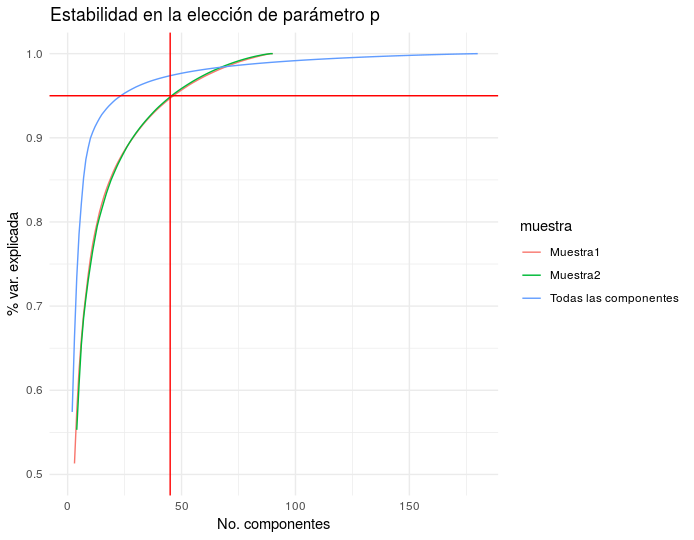
\includegraphics[scale =.7]{eleccion_p_imagenes.png}
    \caption{En esta gráfica podemos ver el porcentaje de varianza explicado acumulado contra el número de componentes de toda la muestra y de dos submuestras (no equilibradas), parece haber un indicio de inestabilidad para $p$. La línea horizontal marca el 95\% de la varianza acumulada, la línea vertical 45 componentes. Con esta $p$ se espera que la varianza explicada en los conjuntos de entrenamiento no esté por debajo del 80\% y 85\%.}
    \label{figura4_1}
  \end{center}
\end{figure}

Consideré un conjunto de entrenamiento del 80\% del tamaño de la muestra para este y el siguiente inciso. Después de una búsqueda manual de los parámetros, pues utilice mi propia implementación de Adaboost, para la clasificación ‘semantic.expression’  logre una precisión de 75\% con los parámetros $M = 100, maxdepth = 10, cp = .0001$ y $ minisplit = 3$. El analisis se anexa en el archivo 'ejercicio4.R' de la carpeta 'tarea4'.

\item \textit{Ahora hazlo considerando las etiquetas \textbf{file.expression.} ¿Qué diferencias notas en
el desempeño?}

Después de una búsqueda manual de los parámetros, pues utilice mi propia implementación de Adaboost, para la clasificación ‘semantic.expression’  logre una precisión de 69\% con los parámetros $M = 50, maxdepth = 10, cp = .0001$ y $ minisplit = 3$. \\
En la figura 4.2 podemos ver como disminuye el error de entrenamiento para AdabOost considerando los dos etiquetamientos de nuestro conjunto de datos, tanto la partición de entrenamiento como la de prueba son las mismas. \\

\begin{figure}[H]
  \begin{center}
    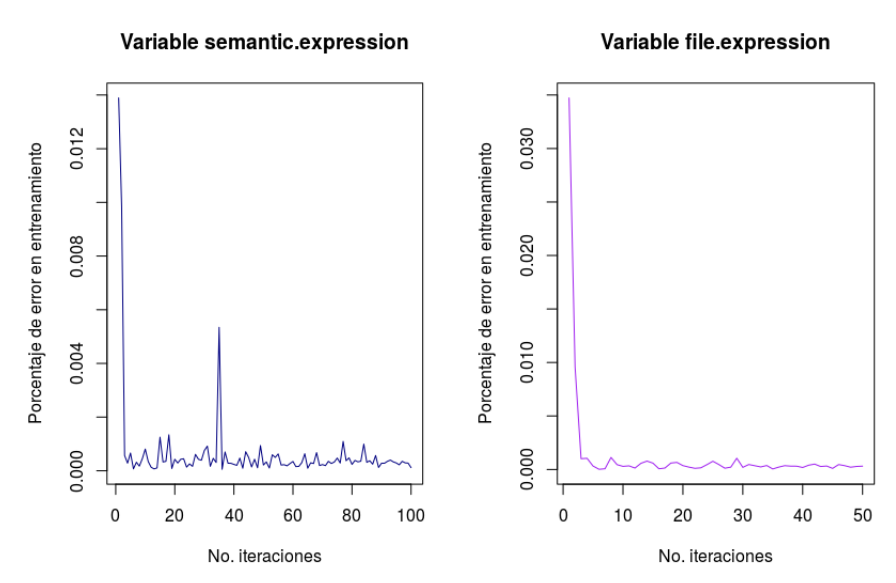
\includegraphics[scale =.5]{EJERCICIO4.jpg}
    \caption{Disminución del error en Adaboost sobre la misma muestra de entrenamiento pero diferentes etiquetas.}
    \label{figura4_2}
  \end{center}
\end{figure}
La diferencia en el desempeño es muy marcada. Al usar file.expression el error de entrenamiento decae rápidamente con la mitad de iteraciones sobre la misma muestra en comparación de la otra etiqueta. Sin embargo con ninguna semilla encontre un escenario donde el modelo con la variable file.expression mejorará al otro. Por lo que infiero que el la propiedad de generalización del modelo file.expresión es menor que la de su competidor. Esto es apoyado por el origen de las etiquetas pues en el caso de file.expression un agente externo jusgó a una persona mientras que en el otro caso la persona se auto diagnóstico, el primer escenario provocaría sesgo que es lo que concluimos.\\



\item  \textit{Prueba el clasificador que elegiste en imágenes tuyas para estimar tu expresión. Prueba con distintos tipos de fondo, luminosidad y posición para verificar qué tan sensible es a las características del entorno.}\\
\begin{figure}[H]
  \begin{center}
    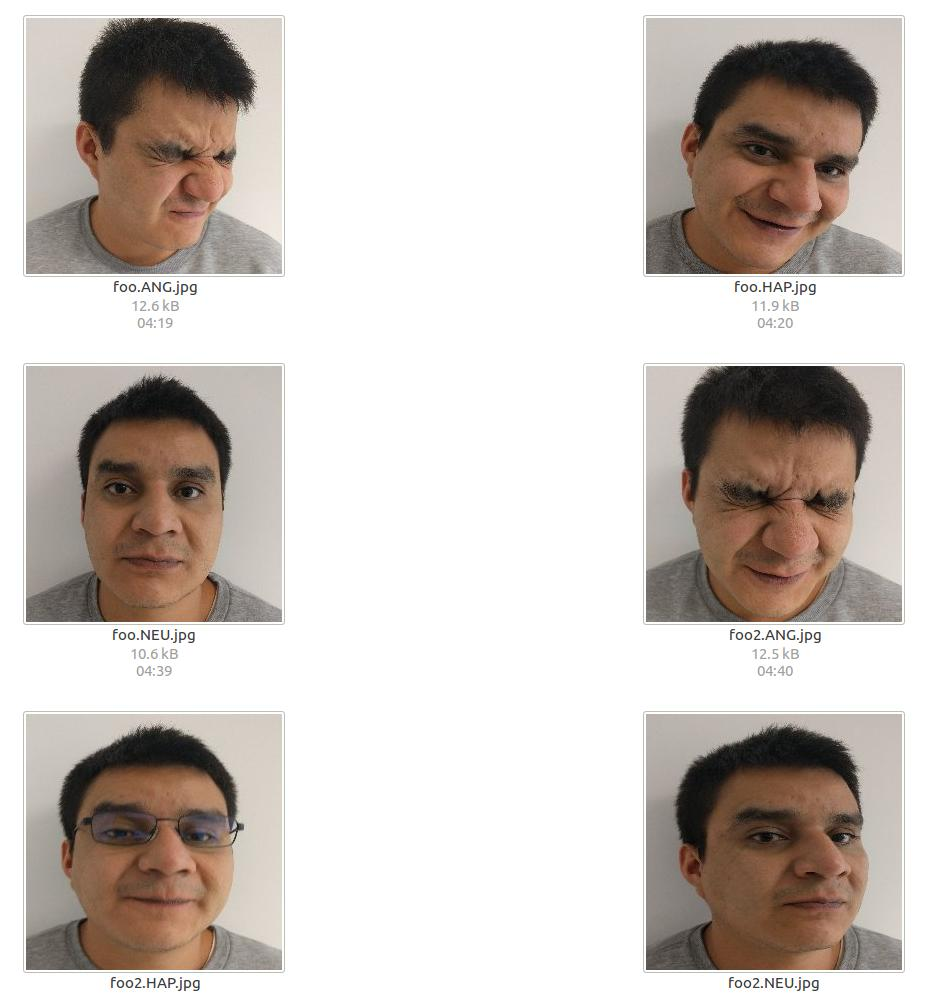
\includegraphics[scale =.3]{fotos.jpg}
    \caption{Conjunto de imágenes con las que se probará el modelo entrenado, nótese que los nombres incluyen la clasificación correspondiente a las contenidas en ‘file.expression’.}
    \label{figura4_3}
  \end{center}
\end{figure}

En la figura 4.3 se muestran las fotos con las que se validará el modelo entrenado anteriormente. en este caso el recorte de las fotos y el redimensionamiento de las mismas se efectuó con la misma herramienta que en el ejercicio 3 sin embargo en este caso no se segmento el fondo. Además las fotos presentan algunas variaciones en intensidad de luz y postura de la cara.\\
Sorprendentemente las seis imágenes fueron clasificadas como ‘DIS’ lo que explicaría por qué la gente suele decir que tengo cara de enojado :D . Podemos notar que las rotaciones y cambios de escala afectan a nuestro clasificador además de que al parecer que la posición de los ojos sea invariante es un requisito fuerte lo que hace que el algoritmo no sea robusto a rotaciones. 





\end{enumerate}
\textit{¿Qué recomendarías para mejorar el clasificador?}\\

Como nuestra ayudante de la clase, Karen , nos comentó alguna vez, las rotaciones afectan a la clasificación de imágenes. Recomendaría buscar tomar las imágenes en condiciones controladas, lo cual es el equivalente a una carta a los reyes magos…, considero que un preprocesamiento más robusto podria quitar ‘ruido en las imagenes’ y por ende suavizar la frontera de clasificación un punto interesante sería encontrar puntos basados en características locales que sean invariantes ante escala (como los SIFT), bajo rotaciones y bajo cambios de intensidad de luz. Si bien en el ejemplo de las frutas omiti que una banda más en la imagen como magnética o alguna longitud de onda diferente a las del espectro visible podrían ayudar a detectar nivel de maduración. En este caso considero que la misma idea es aplicable pues otras bandas-longitudes de onda podrían brindar información de la ‘textura’ del rostro en el sentido de ver que tan estirada o contraída está la piel, tal vez generar un índice sobre ello (como la entropía) puedan mejorar la clasificación.


\section{ Puntos extra: Competencia IMDB}
\textit{
Considera los datos \textbf{movie\_metadata.csv}, que contiene datos extraídos del sitio \textbf{www.imdb.com} de poco mas de 5000 películas. El objetivo es analizar la base de datos y construir métodos de predicción (regresión, clasificación) para dos variables de interés: ganancias (gross) y calificación (\textbf{imdbscore}) de las películas.}
\begin{enumerate}


\item \textit{Utiliza unos métodos para estimar las ganancias basado en las carcateristicas de las películas que consideres 
\textbf{convenientes}. Indica cuál es el criterio que usaste para decidir qué variables utilizar. }\\

Como primer paso identifique las variables continuas (que son 16) y las ordinales (que son 12). Entre las continuas observe que existe poca correlación lineal baja (el colorido correlograma lo presento en el script 'ejercicio6.R'). Y como desconozco la causalidad entre el dinero que recolecta una película y la calificación de imdb descarte esta variable\footnote{Adémas no encontre referencias en la web sobre el conjunto de datos las ur's proporcionadas no tienen soporte ya.}

Por otro lado para todas las variables ordinarias aplique lo aprendido en estadística multivariada (grafique sus respectivos histogramas y verifique que son poco informativos) por lo que decidí realizar un escalamiento multidimensional de las 12 variables ordinales para tener 11 variables continuas (se consiguió un stress 1 de 0.06 para 8 dimensiones obtuve un stress 1 de 0.077, para 7 dimensiones un stress de .1 y para 5 dimensiones un stress de 0.15 por lo que podemos considerar buenas la proyecciones sin enbargo retube solo 7 dimensiones), para la disimilaridad utilice la medida de Gower y el algoritmo SMACOF al graficar en dos dimensiones el resultado del MDS no se observan diferentes grupos sino solo uno y tampoco se observan outliers como se puede apreciar en el código que anexó ‘ejercicio5.R’). \\
Posteriormente realice PCA con los datos estandarizados para determinar un número de componentes principales menores al número de variables continuas, con el cirterio del codo me quede con las primeras 11 componentes principales que explican el 95\% de la varianza total. Teniendo ahora las 11 variables continuas  y las 7 resultado del escalamiento multidimensional. \\

Ya que nuestras variables son ortogonales por grupos, usaremos SVM para realizar la regresión en vista de que ha sido el mejor modelo de clasificación\footnote{Hasta donde recuerdo Vapnik derivó el SVM para regresión en función del SVM para clasificación} el grid sobre el que afinamos $C$ fueron puntos 10 puntos igualmente esparciados en el rango $[0.1, 10]$ las precisiones del modelo obtenidas usando 5-Fold se muestran en la figura 5.1\\


\begin{figure}[H]
  \begin{center}
    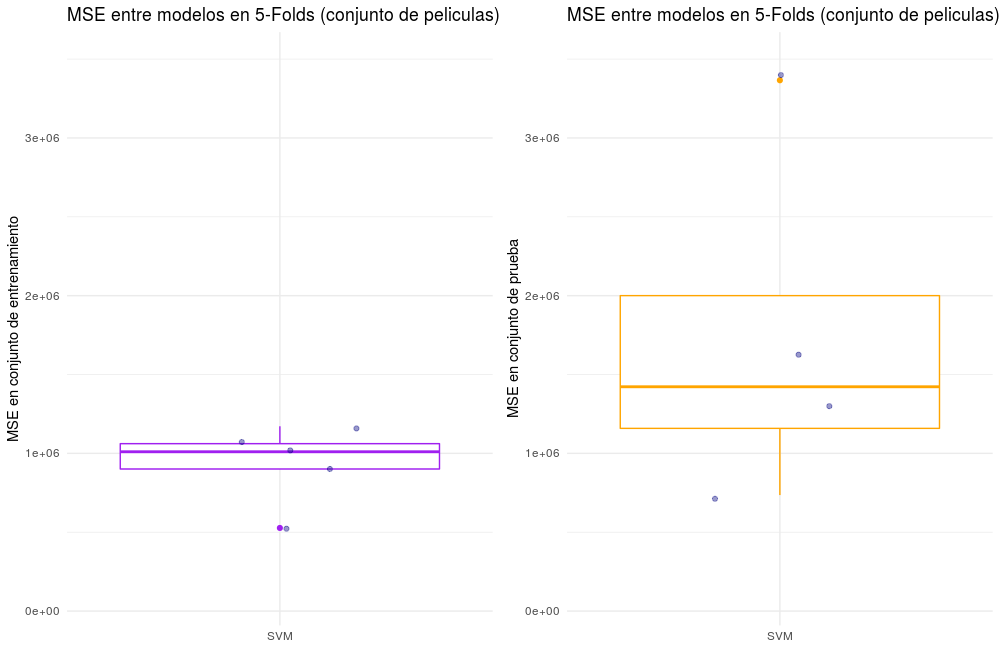
\includegraphics[scale =.7]{SVM5.png}
    \caption{Error cuadratico medio en los conjunto de peliculas de prueba y entrenamiento usando validación 5-Fold SVM. Los puntos representan cada una de las 5 ejecuciones de k-fold, el paámetro $C=1$}
    \label{figura4_1}
  \end{center}
\end{figure}
\end{enumerate}


%\begin{thebibliography}{1}
%\bibitem{Hes}
%Hastie T., Tibshirani R. and Friedman J. , \textit{The Elements of %Statistical Larning}, Springer 2nd., 2009.

%\end{thebibliography}

\end{document}